\chapter{Morpheus Spectral Counter: A Computational Tool for Label-Free Quantitative Mass Spectrometry using the Morpheus Search Engine}

\section{Summary}
Label-free quantitative MS based on the Normalized Spectral Abundance Factor (NSAF) has emerged as a straightforward and robust method to determine the relative abundance of individual proteins within complex mixtures.
Here, we present Morpheus Spectral Counter (MSpC) as the first computational tool that directly calculates NSAF values from output obtained from Morpheus, a fast, open-source, peptide-MS/MS matching engine compatible with high-resolution accurate-mass instruments.
NSAF has distinct advantages over other MS-based quantification methods, including a higher dynamic range as compared to isobaric tags, no requirement to align and re-extract MS1 peaks, and increased speed.
MSpC features an easy to use graphic user interface that additionally calculates both distributed and unique NSAF values to permit analyses of both protein families and isoforms/proteoforms.
MSpC determinations of protein concentration were linear over several orders of magnitude based on the analysis of several high-mass accuracy datasets either obtained from PRIDE or generated with total cell extracts spiked with purified Arabidopsis 20S proteasomes.
The MSpC software was developed in C\# and is open sourced under a permissive license with the code made available at \url{http://dcgemperline.github.io/Morpheus_SpC/}. 

\section{Main Text}
Quantification of individual polypeptides within complex mixtures by MS is an extremely useful tool to understand proteomic changes in organisms during growth and development, and after environmental perturbation \citep{wong10}.
While a number of MS/MS strategies have been developed to measure protein abundance, including Stable Isotope Labeling by Amino Acids in Cell Culture (SILAC), labeling with isobaric tags, and Absolute Quantification of proteins (AQUA) \citep{gerber03, ong02, ross04, thompson03}, label-free quantification (LFQ) have become increasingly popular given their simplicity and low cost \citep{wong10, zhang06}.
One LFQ strategy infers abundance from the number of observed peptide spectra matches (PSMs).
For these PSM-based approaches, changes in protein abundance can be generated artifactually when total PSMs differ among samples and because longer proteins tend to produce more raw counts.
For these reasons normalizing for both protein length and total PSMs is paramount.
While this adjustment can be made in a number of ways; one of the most straight forward methods is to use Normalized Spectral Abundance Factor (NSAF), a length- and count-normalized measure for each protein \citep{zybailov06}.
Further improvements to the NSAF algorithm have been made by accounting for shared peptides in distributed NSAF (dNSAF), which distributes common PSMs among a family of isoforms/proteoforms based on the number of distinct PSMs observed for each isoform/proteoform, and unique NSAF (uNSAF), which ignores shared PSMs and only assigns distinct PSMs to each specific isoform/proteoform \citep{zhang10}.

The Morpheus MS search engine was recently designed for high-resolution, accurate-mass data obtained from Orbitrap-based instruments to provide faster matching of spectra to peptides \citep{wenger13}.
Unfortunately, no downstream automated tools are available to facilitate LFQ analysis, which can be quite challenging, if not impossible, to complete manually when accounting for shared peptides.
To overcome this bottleneck, we developed Morpheus Spectral Counter (MSpC) as the first LFQ computational tool that integrates directly with Morpheus to calculate NSAF, dNSAF, uNSAF, and corrected PSM \citep{fermin11} values in complex protein samples.
\begin{sidewaysfigure}[p]
	\centering
	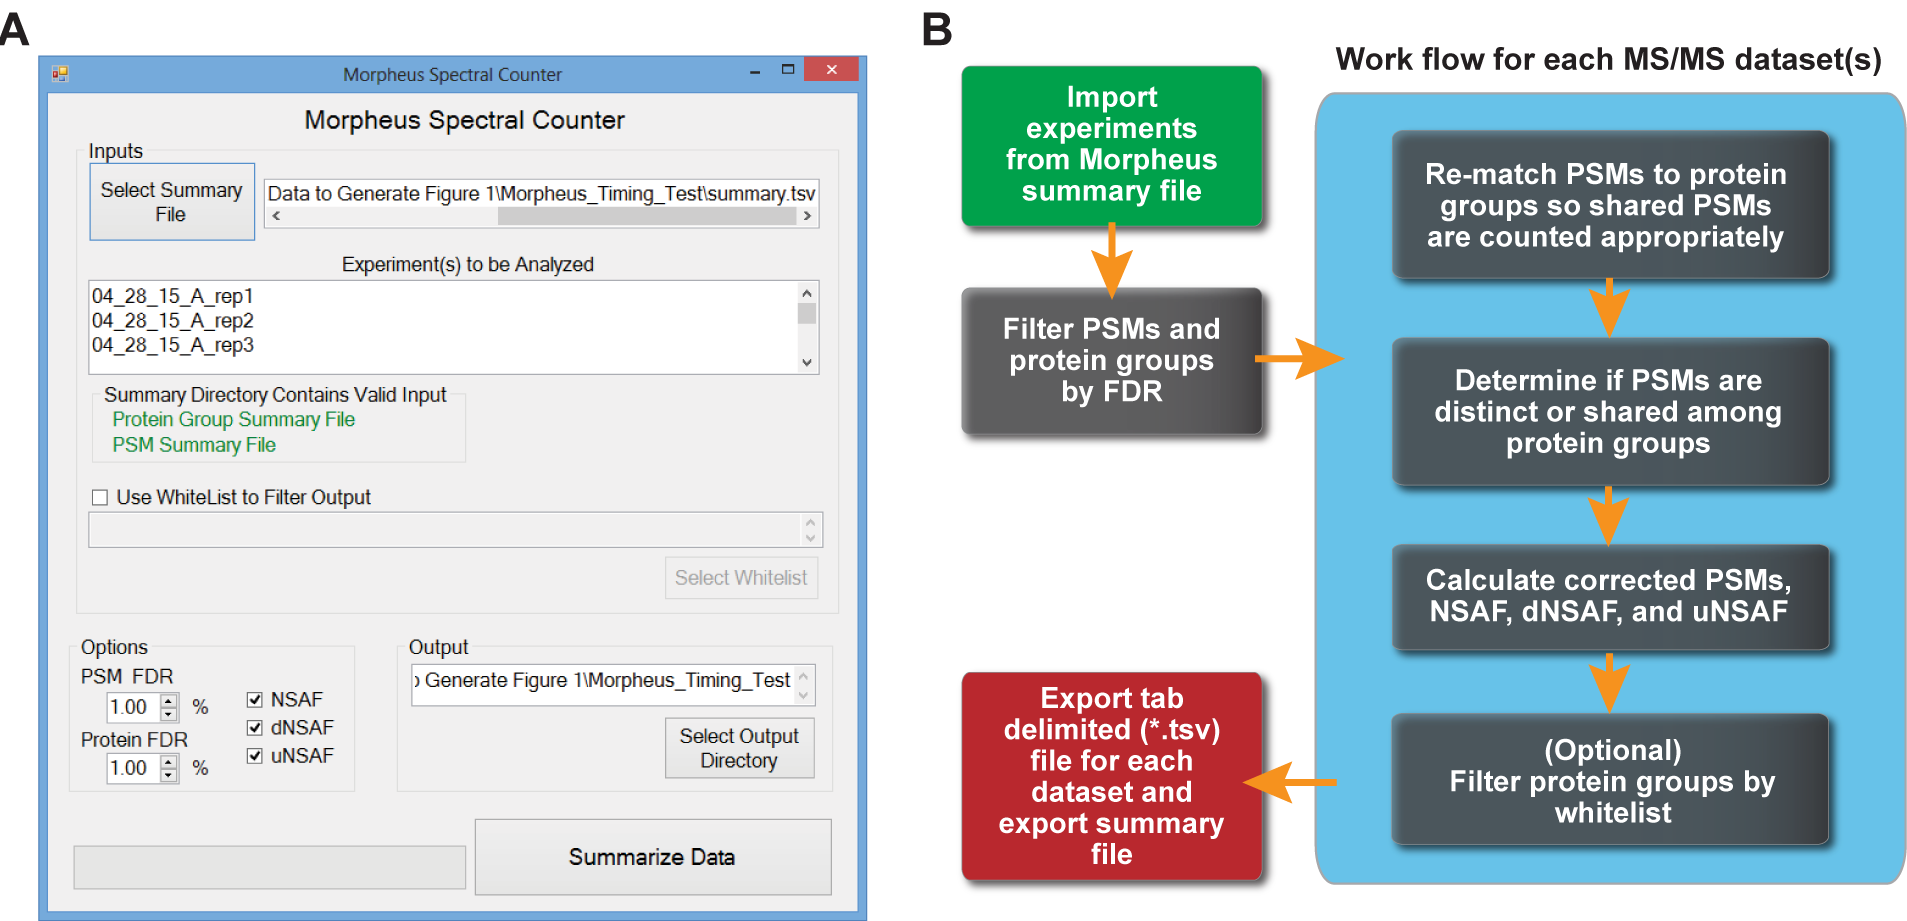
\includegraphics[width=\columnwidth]{MSpC/figure1_supplemental.png}
	\mycaption{MSpC Graphic User Interface (GUI) and software flow chart}{
\textbf(A) Screenshot of the GUI.
The input requires the user to select a Morpheus search summary file containing experiments to be analyzed.  The user can optionally select a whitelist to filter output, and select an output directory.
Additional options can set peptide and protein FDR cutoffs, and method of quantification for output, including Normalized Spectral Abundance Factor (NSAF), distributed NSAF (dNSAF), and unique	NSAF (uNSAF).
A progress bar highlights completion of the analysis.
\textbf(B) Data analysis flow chart.
Experiments and groups of experiments to be analyzed are imported through the Morpheus summary file.
PSMs and protein groups are filtered at the specified FDR cutoff with a default of 1\%.}
	\label{fig:GUIflow}
\end{sidewaysfigure}
MSpC is fully automated, and only requires a Morpheus search summary file (summary.tsv) as input.
The user interface (see Figure \ref{fig:GUIflow} (A)) allows one to select the summary file and displays the raw MS/MS files that will be analyzed by MSpC.
Due to shared peptides being attributed to only one instance of a protein group in Morpheus's PSM file, PSMs are re-matched to all possible protein groups.
PSMs are then cataloged as shared or as unique (distinctly matching one protein group) to generate NSAF, dNSAF, and uNSAF outputs.
Finally, the output can be filtered for proteins of interest by specifying a comma delimited file containing unique identifiers and descriptions.
Some important features of MSpC are its ability to handle fractionation experiments as input, and the ability to whitelist proteins of interest in the output by specifying a csv file (see Tutorial).
Options exist to specify global PSM and protein group FDR rates (thus avoiding increased FDRs when one analyzes many experiments at once), to output NSAF, dNSAF, and uNSAF values, to require a minimum number of unique peptides to quantify a protein, and to specify an output directory.
A progress bar indicates completion of the analysis by MSpC.
To validate the accuracy of MSpC, we analyzed two MS/MS datasets available in PRIDE that were previously generated by high-energy collision-induced dissociation using Thermo Q-Exactive Orbitrap instruments.
\begin{figure}[p]
	\centering
	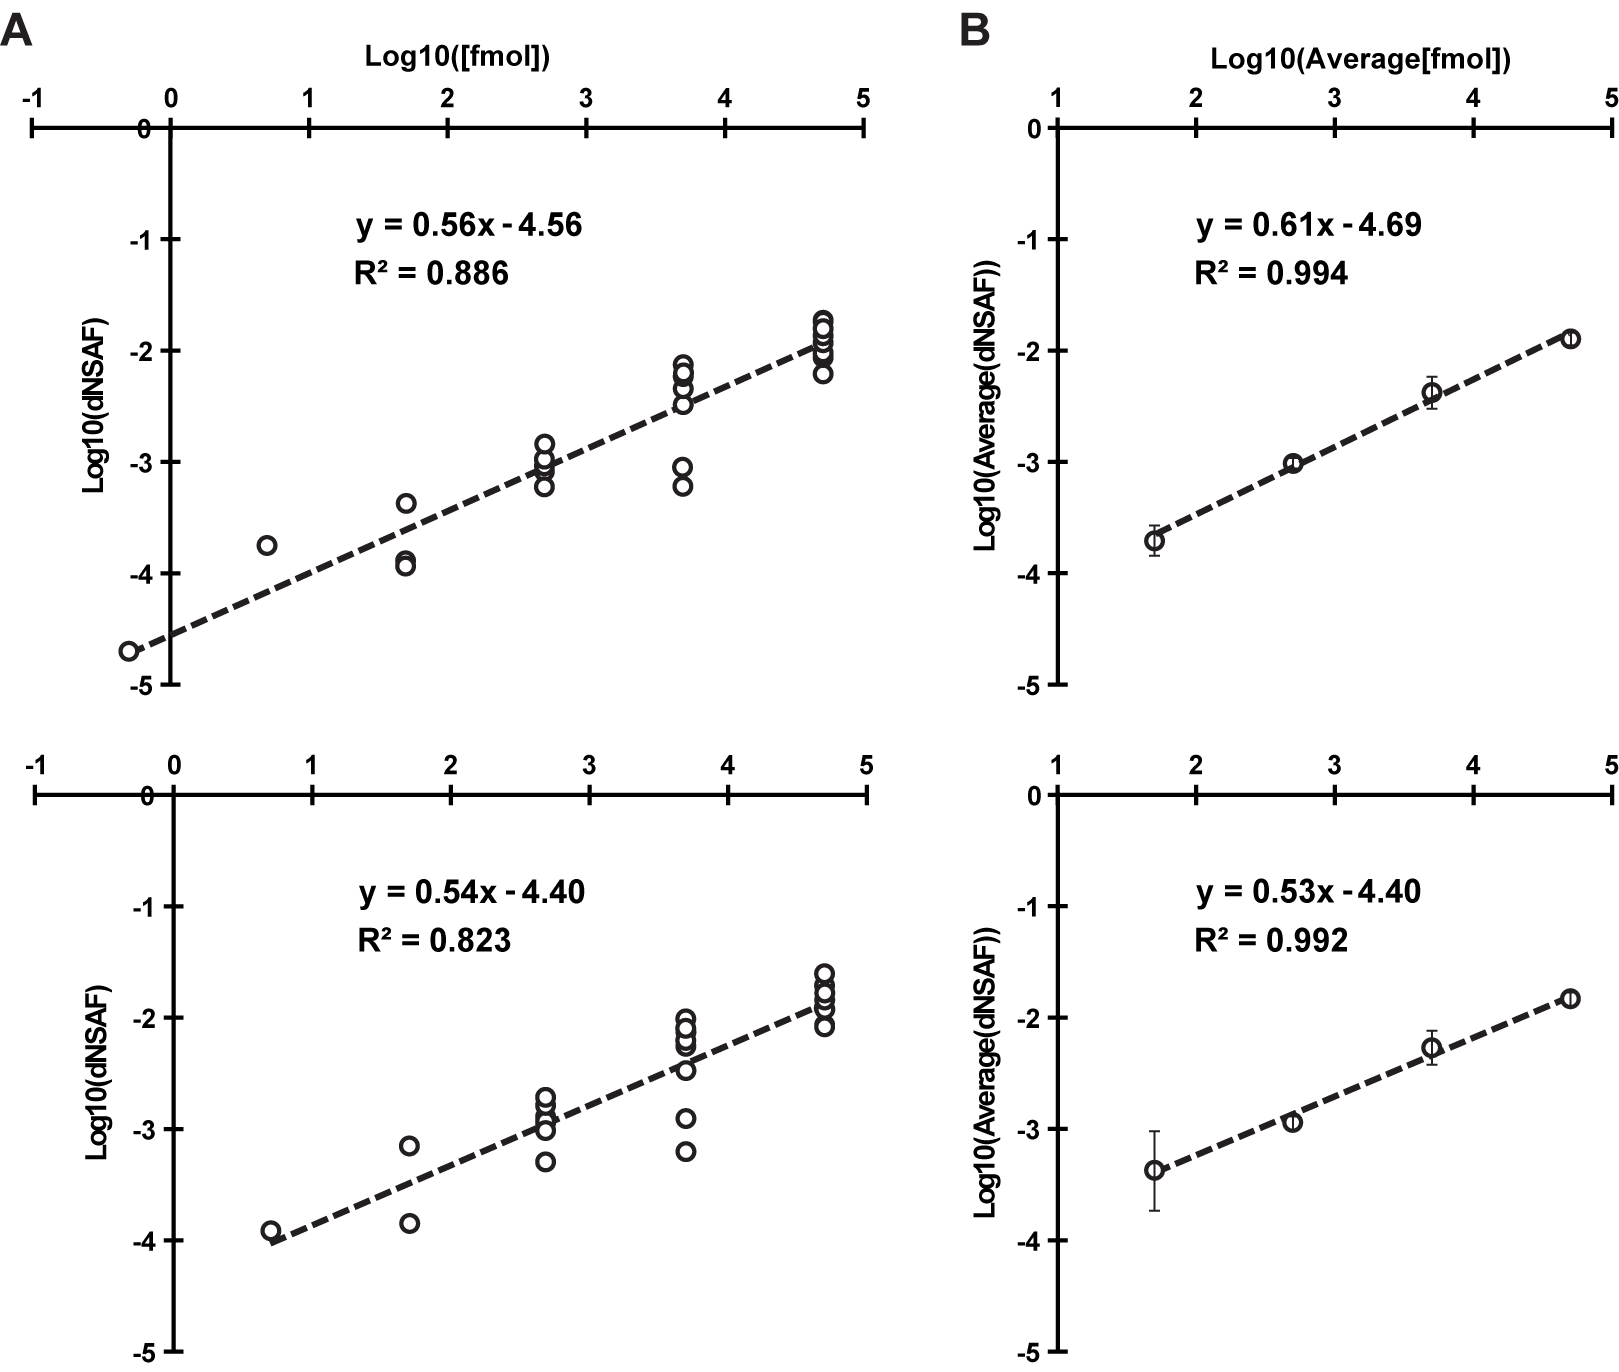
\includegraphics[width=\columnwidth]{MSpC/figure1.png}
	\mycaption{Confirmation of MSpC accuracy by analysis of MS/MS datasets generated with the Universal Proteome Standard 2 (UPS2)}{The array of UPS2 standards were spiked into Xenopus laevis egg \textbf(Top) and embryo \textbf(Bottom) extracts at a range of concentrations.  Following MS/MS analysis, dNSAF values for each protein were determined by Morpheus and MSpC.  \textbf(A) A log-log plot of dNSAF versus concentration for each UPS2 protein detected across each fmol range.  \textbf(B) A log-log plot of average dNSAF vs average concentration of each group of UPS2 proteins at each fmol range: (50, 500, 5000, and 50,000 fmol).}
	\label{fig:UPS2}
\end{figure}

Here, Xenopus egg (see top, Figure \ref{fig:UPS2}) and embryo (bottom, Figure \ref{fig:UPS2}) extracts were spiked at a 4:1 ratio with the Universal Proteome Standard 2 (UPS2), a mix of 48 purified proteins at defined molar ratios of 0.5, 5, 50, 500, 5000, and 50,000, with each ratio containing a different set of 8 of the 48 proteins.
As shown in Figure \ref{fig:UPS2} A, when the Morpheus/MSpC pipeline was used to calculate the average dNSAF value for each UPS2 protein, requiring only a single unique peptide to quantify, strong linear correlations (R$\textsuperscript{2}$ = 0.886 and 0.823) were obtained across a 1,000 fold change in abundance (50 fmol to 50,000 fmol).
In fact, the R$\textsuperscript{2}$ values were similar to those obtained by others with PSM-based LFQ methods \citep{cox14, tu14}.
This linear correlation was further strengthened when the dNSAF values were averaged for all UPS2 proteins within each of the concentration groups, with R$\textsuperscript{2}$ values of 0.994 and 0.992 for the egg and embryo datasets, respectively (see Figure \ref{fig:UPS2} B).
Notably, the slope of the concentration series was significantly less than unity, showing that NSAF measurements are not appropriate for absolute quantification, which was expected given that NSAF is a relative value.  

We also reprocessed the UPS2 dataset using the option of requiring a minimum of two unique peptides for quantification, which should improve stringency.
\begin{figure}[p]
	\centering
	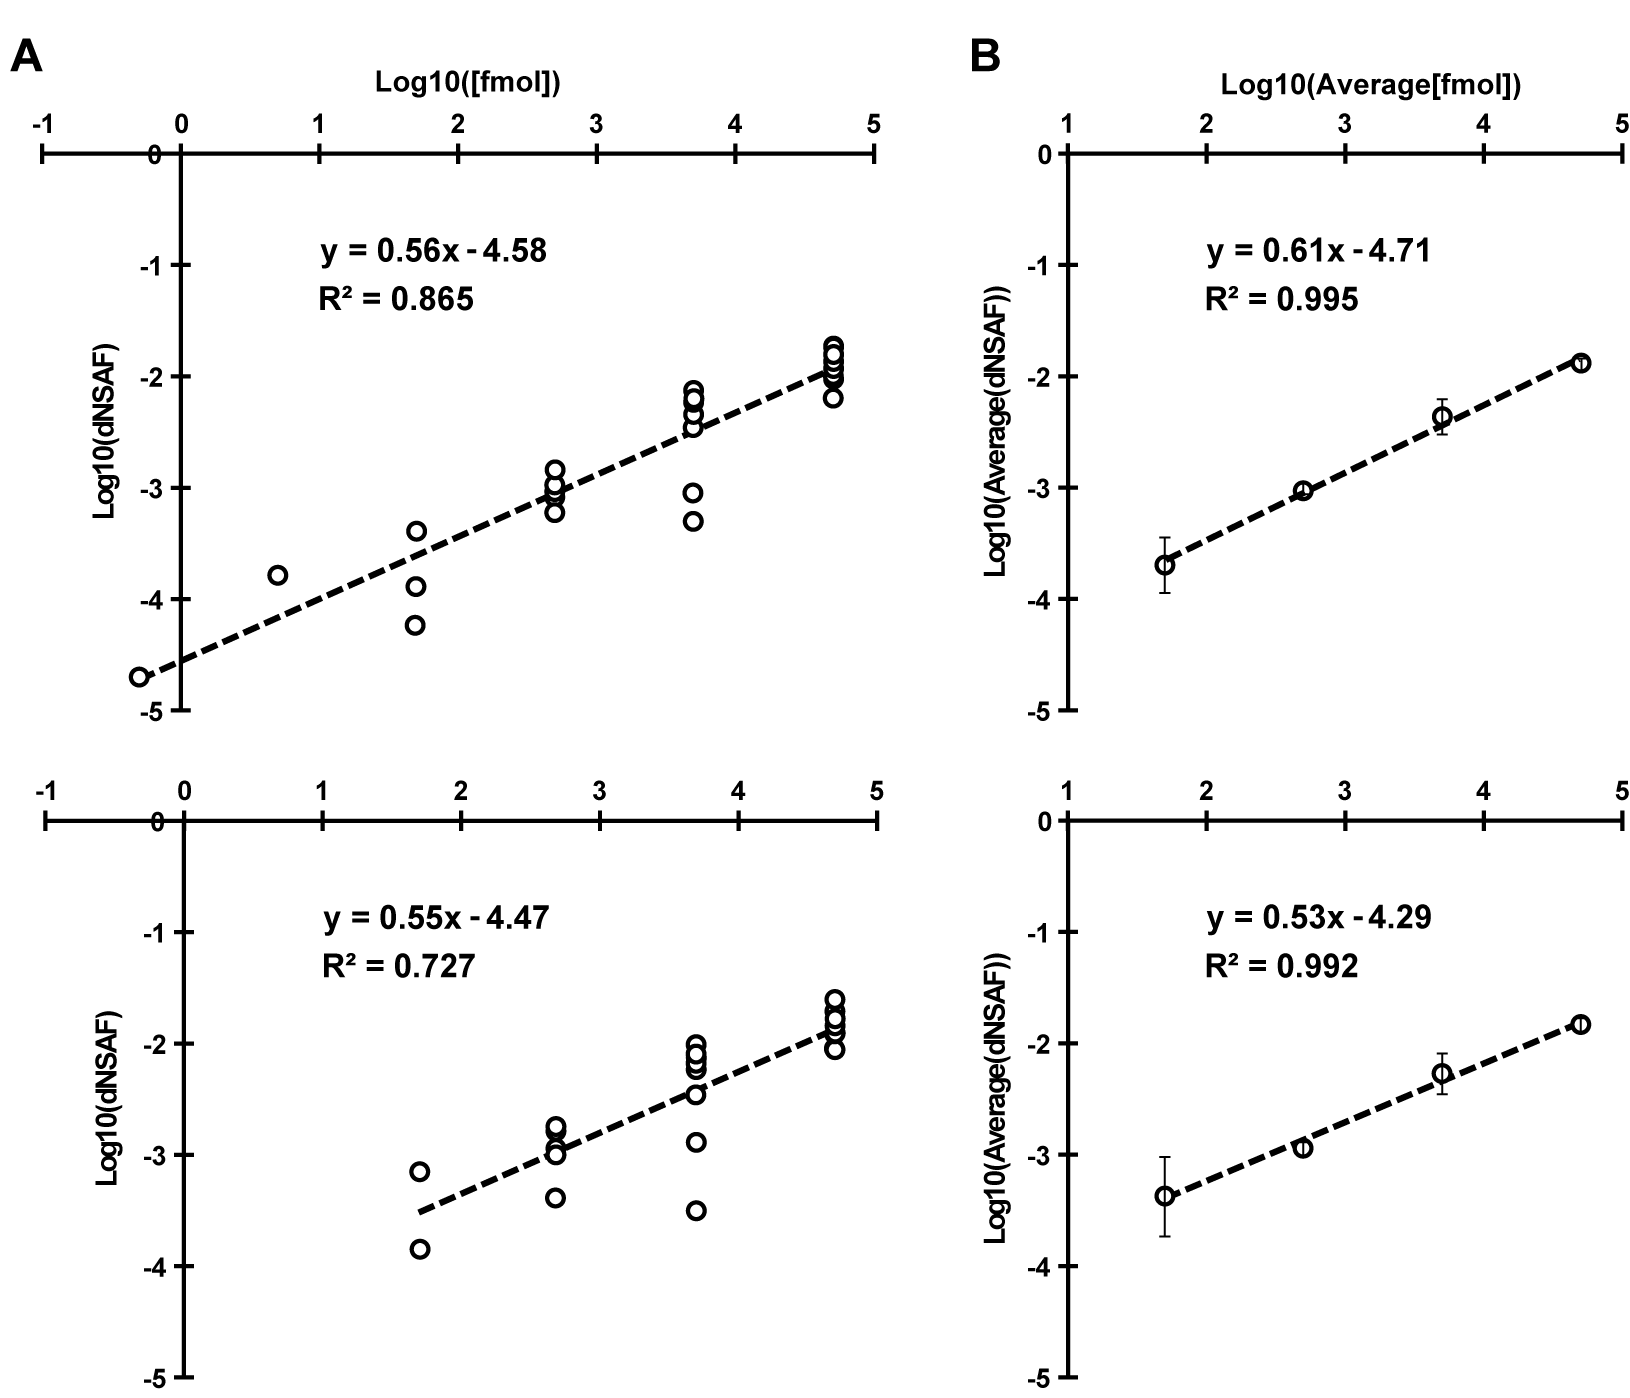
\includegraphics[width=\columnwidth]{MSpC/figure2_supplemental.png}
	\mycaption{Re- Analysis of MS/MS datasets generated with the Universal Proteome Standard 2 (UPS2)}{The array of UPS2 standards were spiked into Xenopus laevis egg \textbf(Top) and embryo \textbf(Bottom) extracts at a range of concentrations.  Following MS/MS analysis, dNSAF values for each protein were determined by Morpheus and MSpC with a change from Figure \ref{fig:UPS2} in that two unique peptides were required to quantify a protein. \textbf(A) A log-log plot of dNSAF versus concentration for each UPS2 protein detected across each fmol range.  \textbf(B) A log-log plot of average dNSAF vs average concentration of each group of UPS2 proteins at each fmol range: (50, 500, 5000, and 50,000 fmol).}
	\label{fig:UPS2twopep}
\end{figure}
This option provided only a minor improvement in overall linearity for the average UPS2 dNSAF values, but decreased linearity when each UPS2 protein was considered individually and removed some UPS2 proteins at low concentrations (compare Figure \ref{fig:UPS2twopep} A to Figure \ref{fig:UPS2} A).
Consequently, caution should be exercised when selecting this option even though it might provide a slight improvement in stringency (see supplemental discussion in Supporting Information).
To demonstrate the utility and accuracy of MSpC as applied to our work, we analyzed 20S proteasomes isolated from Arabidopsis thaliana.
This particle contains multiple subunits assembled in stoichiometric amounts, with many subunits encoded by two paralogous genes of sufficient amino acid identity (typically >90\% \citep{yang04}) such that discrimination between paralogs can be challenging using LFQ approaches \citep{book10}.
To simulate changes in 20S proteasome abundance, we added varying amounts of trypsinized proteasomes (0.05 µg to 3 µg) to a fixed amount of trypsinized E. coli lysate (0.5 µg) to generate proteasome/lysate ratios of \textasciitilde0.091, 0.167, 0.333, 0.500, 0.667, 0.750 0.800, 0.857.
The digests were then subjected to MS/MS and the dNSAF value for each subunit along with the uNSAF value for individual isoforms were calculated by the Morpheus/MSpC pipeline (see Supplemental Methods).
\begin{FPfigure}[Figure \ref{fig:proteasomespike} \textit{caption follows on next page}]
	\centering
	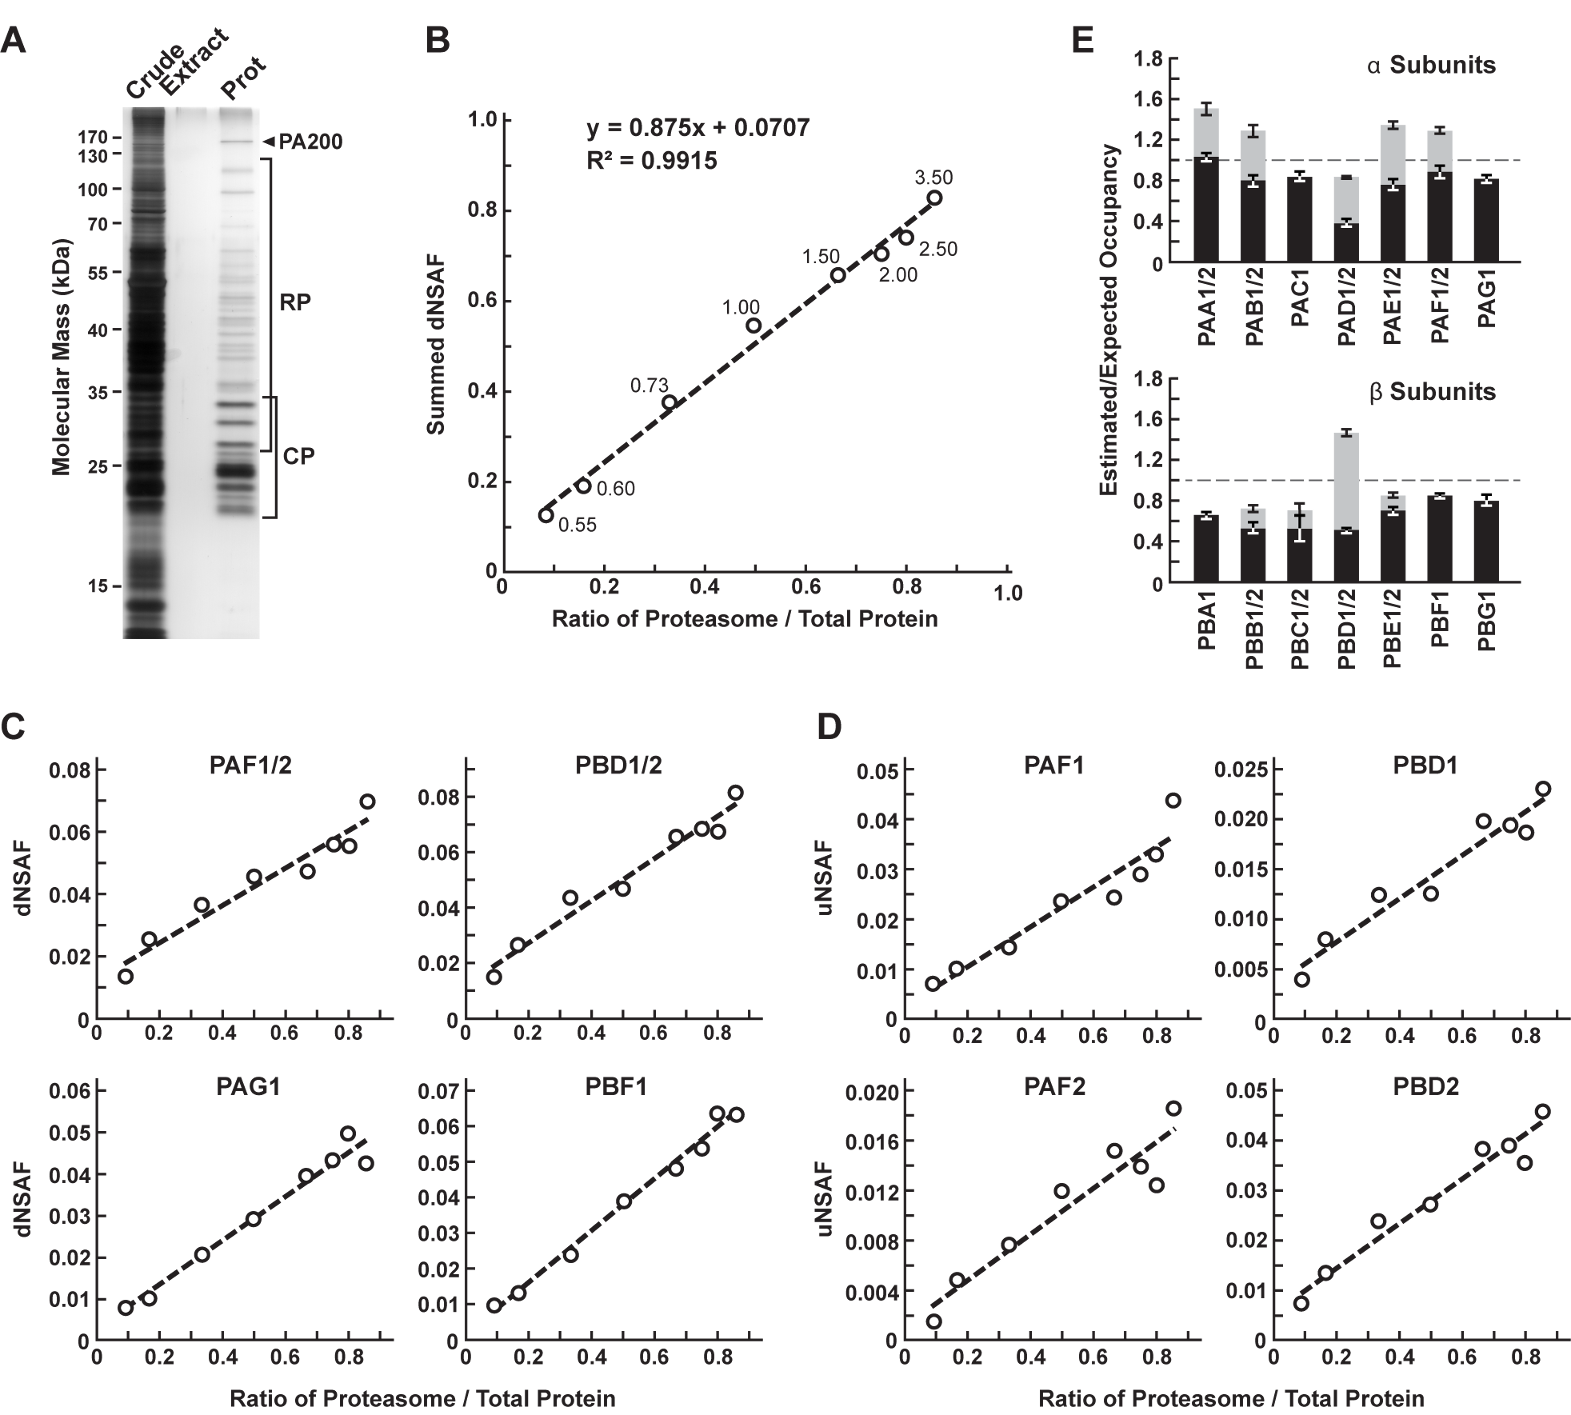
\includegraphics[width=\columnwidth]{MSpC/figure2_rescale.png}
	\mycaption{Confirmation of MSpC accuracy by analysis of MS/MS datasets generated with affinity purified Arabidopsis 20S proteasomes spiked into a total cell lysate from E. coli. Following MS/MS analysis, the dNSAF and uNSAF values for each subunit/isoform were determined by Morpheus and MSpC}
	{\textbf{(A)} A silver-stained SDS-PAGE gel of 20S proteasome samples affinity purified from 10-d-old Arabidopsis seedlings. The crude seedling extract(CE), sample buffer (SB), and affinity-purified 20S proteasome samples (Prot) are shown. \textbf{(B)} Quantification of trypsinized 20S proteasomes when mixed at varying ratios with trypsinized total protein lysates from E. coli. The spiked samples were subjected to MS/MS followed by data analysis with the Morpheus and MSpC. dNSAF values for each proteasome subunit were averaged across three technical replicates, then summed to obtain an estimate of abundance for the 20S proteasome, and plotted against their known ratios. The total protein load is listed at each point in ug. \textbf{(C} and \textbf{D)} dNSAF and uNSAF values determined from the data in panel B for individual subunits \textbf{(C)} and their isoforms {(D)} for several subunits of the 20S proteasome. \textbf{(E)} Quantification accuracy of the Morpheus/MSpC pipeline for determining the amount of each $\alpha$ and $\beta$ subunit of the 20S proteasome. SIngle subunit isoforms are in black, wheras subunits having two isoforms are shown in black and grey to reflect the contributions of isoforms 1 and 2 respectively. Each bar represents the average of eight technical replicates ($\pm$ SE). The dashed line represents the expected value of one assuming an equal stoichiometry of each subunit within the particle.}
	\label{fig:proteasomespike}
\end{FPfigure}
The data from this experiment are deposited in PRIDE with ID PXD003002.
As shown in Figure \ref{fig:proteasomespike}, MSpC provided an excellent determination for the overall abundance of 20S proteasomes within a complex mixture, along with a good reflection of the abundance of individual subunits and their isoforms.
\begin{sidewaystable}
	\centering
	\mycaption{Table of adj\_NSAF values for each 20S proteasome subunit (equivalent to dNSAF) generated by analzying the proteasome spike in experiments with the TPP and ABACUS pipeline}{The top half of the table lists $\alpha$1-7 (PAA-PAG) where 1 or 2 represent different isoforms) subunits, while the bottom half of the table lists $\beta$1-7 subunits (PBA-PBG where 1 or 2 represent different isoforms)}
\npdecimalsign{.}
\nprounddigits{2}
\scalebox{0.7}{
\begin{tabular}{ | l | n{2}{5} | n{2}{5} | n{2}{5} | n{2}{5} | n{2}{5} | n{2}{5} | n{2}{5} | n{2}{5} | l | l | }
\hline
	Ratio & 0.0909090909090909 & 0.166666666666667 & 0.333333333333333 & 0.5 & 0.666666666666667 & 0.75 & 0.8 & 0.857142857142857 &  & Pearsons \\ \hline
	PAA1 & 125.1605 & 166.814933333333 & 245.605733333333 & 355.603 & 491.756533333333 & 494.180766666667 & 504.7474 & 554.9655 &  & 0.987788288683398 \\ \hline
	PAA2 & 57.5179 & 70.5156 & 114.6043 & 126.3541 & 132.057633333333 & 162.254333333333 & 358.126766666667 & 154.6169 &  & 0.493057505529942 \\ \hline
	PAB1 & 96.1281333333333 & 134.976666666667 & 207.903366666667 & 328.155766666667 & 362.214766666667 & 416.455533333333 & 303.600333333333 & 397.3895 &  & 0.865439067273664 \\ \hline
	PAB2 & 29.6656 & 79.4214666666667 & 153.342433333333 & 282.9059 & 365.2214 & 299.465433333333 & 310.191233333333 & 299.9338 &  & 0.848913155268619 \\ \hline
	PAC1 & 95.2721 & 112.4513 & 214.2375 & 376.6589 & 389.0532 & 361.3876 & 512.729966666667 & 488.622566666667 &  & 0.924694988613313 \\ \hline
	PAD1 & 62.5760333333333 & 76.1550666666667 & 106.029166666667 & 196.029166666667 & 179.368066666667 & 182.99 & 164.042 & 188.712266666667 &  & 0.79353639882071 \\ \hline
	PAD2 & 39.8761666666667 & 68.3250666666667 & 145.336133333333 & 178.431866666667 & 190.844066666667 & 246.201933333333 & 243.280033333333 & 240.011133333333 &  & 0.953695573961697 \\ \hline
	PAE1 & 50.4061 & 97.5292333333334 & 193.1804 & 368.874666666667 & 464.7942 & 397.2735 & 468.640233333333 & 534.1594 &  & 0.950854292773049 \\ \hline
	PAE2 & 71.3761666666667 & 80.07 & 184.8455 & 255.9835 & 299.405033333333 & 290.158533333333 & 304.771366666667 & 348.315966666667 &  & 0.954954859737766 \\ \hline
	PAF1 & 132.672866666667 & 179.603633333333 & 207.677133333333 & 253.509366666667 & 253.0449 & 327.109433333333 & 334.728433333333 & 460.761633333333 &  & 0.834748054996771 \\ \hline
	PAF2 & 0 & 0 & 59.6242 & 70.9316666666667 & 111.829833333333 & 80.2913 & 63.0849 & 65.8575666666667 &  & 0.605990529937574 \\ \hline
	PAG1 & 108.09 & 142.817966666667 & 271.1772 & 389.941233333333 & 495.944133333333 & 530.9014 & 632.718566666667 & 540.855366666667 &  & 0.96630247289725 \\ \hline
	 &  &  &  &  &  &  &  &  &  &  \\ \hline
	Ratio & 0.0909090909090909 & 0.166666666666667 & 0.333333333333333 & 0.5 & 0.666666666666667 & 0.75 & 0.8 & 0.857142857142857 &  & Pearsons \\ \hline
	PBA1 & 85.9936333333333 & 113.008066666667 & 208.3785 & 233.442833333333 & 273.504066666667 & 327.2321 & 417.115533333333 & 560.623866666667 &  & 0.850921399221317 \\ \hline
	PBB1 & 47.7680333333333 & 80.6607 & 195.345666666667 & 324.533766666667 & 303.262266666667 & 220.3566 & 200.505533333333 & 216.7744 &  & 0.440413945248165 \\ \hline
	PBB2 & 17.1106 & 4.53546666666667 & 0 & 0 & 21.0460666666667 & 102.5114 & 144.301233333333 & 187.855433333333 &  & 0.618228756945012 \\ \hline
	PBC1 & 27.1930666666667 & 40.6497 & 165.4624 & 345.143866666667 & 364.189333333333 & 386.5929 & 338.4678 & 373.160833333333 &  & 0.885192639364864 \\ \hline
	PBC2 & 10.6414333333333 & 40.6497 & 0 & 55.5816666666667 & 145.43 & 158.895433333333 & 159.744933333333 & 228.051566666667 &  & 0.844980229680132 \\ \hline
	PBD1 & 50.1409333333333 & 94.4576666666667 & 168.575133333333 & 167.5016 & 244.254266666667 & 248.174666666667 & 252.649766666667 & 319.613733333333 &  & 0.945107382530759 \\ \hline
	PBD2 & 81.4452333333333 & 149.2844 & 256.881833333333 & 319.8908 & 390.595466666667 & 407.019033333333 & 380.297266666667 & 490.1709 &  & 0.950089780554562 \\ \hline
	PBE1 & 81.0115333333333 & 107.7629 & 196.210233333333 & 302.899566666667 & 365.0328 & 404.247133333333 & 378.6655 & 441.0343 &  & 0.981079214776472 \\ \hline
	PBE2 & 0 & 1.51736666666667 & 5.592 & 8.04916666666667 & 40.0649 & 56.5627666666667 & 59.3858 & 58.5621 &  & 0.886783231269529 \\ \hline
	PBF1 & 71.5308 & 112.260333333333 & 190.453766666667 & 226.886666666667 & 259.900866666667 & 366.597233333333 & 431.420033333333 & 420.228533333333 &  & 0.94257878462495 \\ \hline
	PBG1 & 104.9337 & 174.549766666667 & 232.341733333333 & 392.370766666667 & 425.101 & 397.848 & 396.4215 & 463.1298 &  & 0.905749458006341 \\ \hline
	 &  &  &  &  &  &  &  &  &  &  \\ \hline
	 &  &  &  &  &  &  &  &  & Average & 0.844830435248515 \\ \hline
\end{tabular}}
\npnoround
\label{table:abacus}
\end{sidewaystable}
When the dNSAF values for all subunits for the Arabidopsis 20S proteasome including their isoforms (representing 14 distinct subunits, 10 of which exist as isoform pairs) were summed, a very close approximation of the dNSAF/actual abundance was obtained (slope=0.875) with a very strong linear correlation (R$\textsuperscript{2}$ = 0.99) over a \textasciitilde10-fold range in protein abundance.  
When each 20S proteasome subunit was analyzed individually, a strong linear response was also obtained (R$\textsuperscript{2}$ > 0.90) for a majority of subunits (Figure \ref{fig:proteasomespike} C and Supplemental Table 1).

For example, reasonably accurate concentration plots were obtained for the PAF ($\alpha$6) and PBD ($\beta$4) subunits that are encoded by the PAF1/2 and PBF1/2 gene pairs, and for the PAG ($\alpha$7) and PBF ($\beta$6) subunits that are encoded by single PAG1 and PBF1 genes (R$\textsuperscript{2}$  from 0.94 to 0.99).
Even when we calculated uNSAF values for individual isoforms added to the E. coli lysate, strong linear responses were obtained (e.g., the PAF1/PAF2 and PBD1/PBD2 pairs) with robust correlations (R$\textsuperscript{2}$ from 0.89 to 0.95) (Figure 2D).
Taken together, MSpC worked well for relative LFQ analysis of a multi-subunit complex and its individual subunits and isoforms within a complex proteomic mixture.

The Morpheus/MSpC pipeline also allowed us to calculate the respective incorporation of each paralog in the complex (see Supplemental Methods).
As shown in Figure 2E, these estimated/expected occupancies were close to unity for most subunits within both the $\alpha$ and $\beta$ rings of the 20S proteasome.
The only strong deviation was for PBD1/2 ($\beta$4), which  had a greater dNSAF value relative to other $\beta$ subunits across the experiments analyzed (Supplemental Table 1).
The calculations for uNSAF values also estimated the relative proportion of each isoform within the complex for those subunits expressed from paralogous genes.
The data obtained are similar to prior studies of the complex involving quantitative top-down proteomic analysis of purified proteasome samples using ultra violet-intrinsic fluorescence to quantify tyrosine-containing subunits \citep{russell13}.
However, our MSpC analysis provided a more complete picture as several subunit isoforms were difficult to quantify by fluorescence either because they lacked tryosine, or because their fluorescence peaks overlapped with those of other subunits/isoforms.
Notably , the protein isoform ratios measured here agree well with the expression ratios for the paralogous genes \citep{book10}, suggesting that the protein isoform abundance generally reflects the relative transcriptional activity of the gene pair.
We consistently estimated slightly more $\alpha$ ring subunits (PAA-PAG) versus $\beta$ ring subunits (PBA-PBG) in the final MSpC calculations (Figure 2E).
This deviation could represent enhanced detection of $\alpha$ ring versus $\beta$ ring subunits, or more likely that purification via the tagged $\alpha$ ring subunit PAG1 also isolated assembly intermediates comprised of only $\alpha$ ring subunits.

We compared the Morpheus and MSpC pipeline to the next most comparable open source, spectral-count-based LFQ pipeline, The Trans Proteomic Pipeline (TPP) \citep{deutsch10} and ABACUS \citep{fermin11} using our datasets generated with the 20S proteasome/E. coli lysate mixture (Supplemental Table 1 and 2).
Morpheus/MSpC slightly outperformed TPP/ABACUS by having a greater overall accuracy (average linearity of 0.88 compared to 0.84), and by having more subunits showing an R$\textsuperscript{2}$ linear correlation greater than 0.9 (14/23 subunits for MSpC versus and 11/23 for ABACUS).
In addition to this modest improvement, we note that the Morpheus/MSpC pipeline required significantly less intermediary steps, thus accelerating the data analysis.
Some of the additional steps in TPP/ABACUS could be automated from the command-line, but it would likely be a challenge for the average user.
Importantly, we found that the Morpheus/MSpC pipeline was faster.
Timing tests using the proteasome/E. coli spike data generated here showed that the Morpheus/MSpC pipeline was 1.9-fold faster than the TPP/ABACUS pipeline (Figure 3).
Such an improvement was expected given that Morpheus completes its searches on average 1.3 to 4.6 times faster than most other search engines available \citep{wenger13}. 
Given its simplicity of use, speed, and open source nature, MSpC combined with Morpheus is clearly advantageous over other PSM-based LFQ approaches currently available.  Moreover, by being open source, MSpC should allow others to extend its utility and to serve as a platform for integrating additional open source LFQ approaches into the Morpheus pipeline. 

\section {Methods}

\section {Tutorial}

\section {Acknowledgements}
D.C.G. was supported by a grant from the U.S. Department of Energy Office of Science; Office of Basic Energy Sciences; Chemical Sciences, Geosciences, and Biosciences Division (DE-FG02-88ER13968) and a graduate training fellowship from the NIH (5 T32 GM 7133-37).  M.S. and L.M.S were supported by a grant from the National Institute of Health/National Institute of General Medical Sciences (1P50HG004942).  The authors thank Erin Gemperline, Richard S. Marshall, and Josh Coon for critical reading of the manuscript, and additionally thank Derek Bailey for a critical code review.

\bibliographystyle{plantcell2}
\bibliography{MSpC}
